\section{Addition}
\label{sec:add}

Addition is the simplest of the basic arithmetic operators. It is a cornerstone
that can be used to define all other operations - an essential part of every
arithmetic.

Former work has been carried out for addition in Futhark, which will serve as a
stepping stone for the algorithm and implementation of our addition
\cite{DPPproject}. In essence, big integer addition formalizes to a 
\texttt{map}-\texttt{scan} composition, making it run efficiently on a GPGPU
\cite{blellochaddscan}.

This section is structured as follows: In \ref{subsec:addalg} we present a
parallel algorithm to compute big integer addition. In \ref{subsec:addcud} and
\ref{subsec:addfut} we discuss how to efficiently implement the algorithm in
CUDA and Futhark, respectively. Lastly, in \ref{subsec:sub} we show how to
define subtraction from the addition algorithm.

\subsection{Algorithm}
\label{subsec:addalg}
From the Definition \ref{def:bigints} we derive the following addition definition.

\begin{definition}[big integer addition]
  The addition of two big integers $u$ and $v$ of size $m$ and base $B$ is the
  sum of their added digits:
\begin{equation}
  \label{eq:add}
  u + v  = \sum_{i=0}^{m-1}(u_i+v_i) B^{i}
\end{equation}
\end{definition}

I.e.\ we compute each digit of the result simply by adding the corresponding two
input digits. However, these inner additions may overflow the base, resulting in
a carry being added to the following digit. In turn, this digit may now
overflow, and so we need to add yet another carry, and so forth. E.g.\ consider
the addition $199 + 1$ of decimal base; first we add $1$ to $9$ giving $0$ and a
carry, then we add $0$ and the carry to $9$ giving $0$ and another carry, which
we then add to $1$, resulting in the number $200$:
{\scriptsize
\begin{tabular}{cccc}
  & \scalebox{.62}{1} & \scalebox{.62}{1} & \\[-0.7ex]
  & 0  & 0 & 1 \\[-0.5ex]
+ & 1  & 9 & 9 \\[-0.4ex]
\hline
  & 2 & 0 & 0 \\
\end{tabular}
}

A sequential algorithm, and illustration thereof, is given in Figure
\ref{fig:addseq}. It is immediate from the figure that the sum of digits can be
independently computed, and thus, trivially parallelizable. However, the carries
are truly dependent on all sums and carries before it, as illustrated in the
figure, but we know they can be computed using a \texttt{scan}
\cite{blellochaddscan}.

\begin{figure}
  \centering
  \begin{minipage}{0.45\textwidth}
    \small
    \texttt{Input:} $u$ and $v$ of size $m$ base $B$\\
    \texttt{Output:} $w$ of size $m$ in base $B$
\begin{lstlisting}[language=pseudo,frame=]
c = 0
for i in (0..m-1)
    w[i] = u[i] + v[i] + c
    c = if overflow then 1 else 0
\end{lstlisting}
  \end{minipage}
  \begin{minipage}{0.45\textwidth}
    \centering
    \footnotesize
    \begin{tabular}{c}
      \begin{tabular}{|C{0.7cm}|C{0.7cm}|C{0.7cm}|C{0.7cm}|C{0.7cm}|}
        \hline
        $u_0$ & $u_1$ & $u_2$ & $\cdots$ & $u_{m-1}$\\ 
        \hline
      \end{tabular}\\
      \begin{tabular}{C{0.7cm}C{0.7cm}C{0.7cm}C{0.7cm}C{0.7cm}}
        $+$ & $+$ & $+$ & & $+$\\ 
      \end{tabular}\\
      \begin{tabular}{|C{0.7cm}|C{0.7cm}|C{0.7cm}|C{0.7cm}|C{0.7cm}|}
        \hline
        $v_0$ & $v_1$ & $v_2$ & $\cdots$ & $v_{m-1}$\\
        \hline
      \end{tabular}\\
      \begin{tabular}{C{0.7cm}C{0.7cm}C{0.7cm}C{0.7cm}C{0.7cm}}
        $+$ & $+$ & $+$ &  & $+$\\
      \end{tabular}\\
      \begin{tabular}{C{0.7cm}C{0.7cm}C{0.7cm}C{0.7cm}C{0.7cm}}
        $0$ & $c_0$ &  $c_1$ & $\cdots$ &$c_{m-2}$ \\
      \end{tabular}\\[-0.8ex]
      \begin{tabular}{C{0.15cm}C{0.15cm}C{0.15cm}C{0.15cm}C{0.15cm}C{0.15cm}C{0.15cm}}
       \diagonalarrow{} & & \diagonalarrow{} &  & \diagonalarrow{} &  & \diagonalarrow{}\\
      \end{tabular}\\[-2ex]
      \begin{tabular}{C{0.7cm}C{0.7cm}C{0.8cm}C{0.7cm}C{0.7cm}}
        $=$ & $=$ & $=$ &  & $=$  
      \end{tabular}\\
      \begin{tabular}{|C{0.7cm}|C{0.7cm}|C{0.7cm}|C{0.7cm}|C{0.7cm}|}
        \hline
        $w_{0}$ & $w_1$ & $w_2$ & $\cdots$ & $w_{m-1}$\\
        \hline
      \end{tabular}
    \end{tabular}
  \end{minipage}
  \caption{\footnotesize Pseudo-code and illustration of sequential addition algorithm.}
  \label{fig:addseq}
\end{figure}

Each addition may overflow once at most, and so we need to figure out the
conditions for an overflow. In the former work by Olesen, Topalovic and
Restelli-Nielsen, they found that this happens when I) the addition already
overflowed, or II) it results in the maximum representable integer, and the
addition just before it overflowed \cite{DPPproject}. They found that these
conditions can efficiently be checked in parallel as a prefix
sum.\footnote{Specifically an exclusive prefix-sum, which is easy to see on the
  arrows in Figure \ref{fig:addseq}.}

Thus, the big integer addition parallelizes to a \fun{map}-\fun{scan} function
composition. Figure \ref{fig:addpar} lists and illustrates a generalized
parallel addition algorithm. The algorithm has three steps:
\begin{enumerate}
\item Compute the inner sums (\texttt{r}) and the augmented carries (\texttt{a})
  by mapping operator
  $\oplus:\tau \shortrightarrow \tau \shortrightarrow \tup{\tau}{\tau'}$ over the inputs. The
  augmented carries corresponds to the two conditions from \cite{DPPproject}.
  
\item Propagate the carries by computing the exclusive prefix sum over the
  augmented carries (\texttt{c}) using operator $\otimes:\tau' \shortrightarrow \tau' \shortrightarrow \tau'$ with left-associative
  neutral element $\mathtt{e}:\tau'$.

\item Compress the propagated augmented carries using
  $f:\tau' \shortrightarrow \tau$ and distribute them over the inner sums.
\end{enumerate}

\begin{figure}
  \centering
  \begin{minipage}{0.47\textwidth}
    \footnotesize
    \texttt{Input:} $u$ and $v$ of size $m$ base $B$\\
    \texttt{Output:} $w$ of size $m$ in base $B$\\
    \texttt{Use:} $f$ to extract carry from augmented carry
\begin{lstlisting}[language=pseudo,frame=,escapeinside={(*}{*)},name=paradd,backgroundcolor=\color{LightGray},]
(r, a) = map2 (*$\oplus$*) u v
\end{lstlisting}
\vspace{-\baselineskip}
\begin{lstlisting}[language=pseudo,frame=,escapeinside={(*}{*)},name=paradd,backgroundcolor=\color{Beige}]
c = scan_exc (*$\otimes$*) e a
\end{lstlisting}
\vspace{-\baselineskip}
\begin{lstlisting}[language=pseudo,frame=,escapeinside={(*}{*)},name=paradd,backgroundcolor=\color{LightSteelBlue}]
w = map2 ((*$\lambda$*) x y (*$\rightarrow$*) x + f y) r c
\end{lstlisting}
\end{minipage}
  \noindent\fcolorbox{white}{LightGray}{%
  \begin{minipage}{0.47\textwidth}
    \centering
    \footnotesize
    \begin{tabular}{c}
      \begin{tabular}{|C{0.7cm}|C{0.7cm}|C{0.7cm}|C{0.7cm}|C{0.7cm}|}
        \hline
        $u_0$ & $u_1$ & $u_2$ & $\cdots$ & $u_{m-1}$\\ 
        \hline
      \end{tabular}\\
      \begin{tabular}{C{0.7cm}C{0.7cm}C{0.7cm}C{0.7cm}C{0.7cm}}
        $\oplus$ & $\oplus$ & $\oplus$ & & $\oplus$\\ 
      \end{tabular}\\
      \begin{tabular}{|C{0.7cm}|C{0.7cm}|C{0.7cm}|C{0.7cm}|C{0.7cm}|}
        \hline
        $v_0$ & $v_1$ & $v_2$ & $\cdots$ & $v_{m-1}$\\
        \hline
      \end{tabular}\\
      \begin{tabular}{C{0.7cm}C{0.7cm}C{0.8cm}C{0.7cm}C{0.7cm}}
        $=$ & $=$ & $=$ &  & $=$  
      \end{tabular}\\
      \begin{tabular}{|C{0.7cm}|C{0.7cm}|C{0.7cm}|C{0.7cm}|C{0.7cm}|}
        \hline
        $r_{0}$ & $r_1$ & $r_2$ & $\cdots$ & $r_{m-1}$\\
        \hline
      \end{tabular}\\
      \begin{tabular}{C{0.15cm}C{0.15cm}C{0.15cm}C{0.15cm}C{0.15cm}C{0.15cm}C{0.15cm}}
        & &  &  &  &  & \\
      \end{tabular}\\[-2ex]
      \begin{tabular}{|C{0.7cm}|C{0.7cm}|C{0.7cm}|C{0.7cm}|C{0.7cm}|}
        \hline
        $a_{0}$ & $a_1$ & $a_2$ & $\cdots$ & $a_{m-1}$\\
        \hline
      \end{tabular}\\
    \end{tabular}
  \end{minipage}
  }\\
  \noindent\fcolorbox{white}{Beige}{%
    \begin{minipage}{0.4525\textwidth}
    \centering
    \scriptsize
    \begin{tabular}{c}
      \begin{tabular}{|C{0.7cm}|C{0.7cm}|C{0.7cm}|C{0.7cm}|C{0.7cm}|}
        \hline
        $a_{0}$ & $a_1$ & $a_2$ & $\cdots$ & $a_{m-1}$\\
        \hline
      \end{tabular}\\
      \begin{tabular}{C{0.15cm}C{0.15cm}C{0.15cm}C{0.15cm}C{0.15cm}C{0.15cm}C{0.15cm}C{0.15cm}C{0.15cm}C{0.15cm}C{0.15cm}}
        \texttt{e}$\shortrightarrow$ & $\otimes$ & $\shortrightarrow$ & $\otimes$ & $\shortrightarrow$ & $\otimes$ & $\shortrightarrow$ & $\otimes$ & $\shortrightarrow$ & $\otimes$ & \\
      \end{tabular}\\[-1.2ex]
      \begin{tabular}{C{0.15cm}C{0.15cm}C{0.15cm}C{0.15cm}C{0.15cm}C{0.15cm}C{0.15cm}C{0.15cm}C{0.15cm}C{0.15cm}C{0.15cm}}
       \diagonalarrowdown{} & & \diagonalarrowdown{} & & \diagonalarrowdown{} &  & \diagonalarrowdown{} &  & \diagonalarrowdown{} & &\\
      \end{tabular}\\[-0.3ex]
      \begin{tabular}{|C{0.7cm}|C{0.7cm}|C{0.7cm}|C{0.7cm}|C{0.7cm}|}
        \hline
        $c_{0}$ & $c_1$ & $c_2$ & $\cdots$ & $c_{m-1}$\\
        \hline
      \end{tabular}
    \end{tabular}
  \end{minipage}
}
\noindent\fcolorbox{white}{LightSteelBlue}{%
  \begin{minipage}{0.47\textwidth}
    \centering
    \footnotesize
    \begin{tabular}{c}
      \begin{tabular}{|C{0.7cm}|C{0.7cm}|C{0.7cm}|C{0.7cm}|C{0.7cm}|}
        \hline
        $r_0$ & $r_1$ & $r_2$ & $\cdots$ & $r_{m-1}$\\ 
        \hline
      \end{tabular}\\
      \begin{tabular}{C{0.7cm}C{0.7cm}C{0.7cm}C{0.7cm}C{0.7cm}}
        $\lambda$ & $\lambda$ & $\lambda$ & & $\lambda$\\ 
      \end{tabular}\\
      \begin{tabular}{|C{0.7cm}|C{0.7cm}|C{0.7cm}|C{0.7cm}|C{0.7cm}|}
        \hline
        $c_0$ & $c_1$ & $c_2$ & $\cdots$ & $c_{m-1}$\\
        \hline
      \end{tabular}\\
      \begin{tabular}{C{0.7cm}C{0.7cm}C{0.8cm}C{0.7cm}C{0.7cm}}
        $=$ & $=$ & $=$ &  & $=$  
      \end{tabular}\\
      \begin{tabular}{|C{0.7cm}|C{0.7cm}|C{0.7cm}|C{0.7cm}|C{0.7cm}|}
        \hline
        $w_{0}$ & $w_1$ & $w_2$ & $\cdots$ & $w_{m-1}$\\
        \hline
      \end{tabular}\\
    \end{tabular}
  \end{minipage}
  }
  \caption{\footnotesize Pseudo-code and illustration of parallel addition algorithm.}
  \label{fig:addpar}
\end{figure}

Now, we must figure out what $\oplus$, $\otimes$, \texttt{e} and $f$ is. Olesen et
al.\ found $\oplus$ to augment the carries as a pair of boolean values, encoding the
two conditions straightforward. I.e.\ for digits $x$ and $y$ of type
\texttt{uint} in base $B$ with wrap-around semantics on overflow, we have:
\begin{equation}
\label{eq:oplus}
x \oplus y \coloneq \tup{x + y}{\tup{x + y < x}{x + y == B-1}}
\end{equation}
The first element of the tuple encodes the actual overflows (condition I), and
the second element is the augmented data needed for scanning (condition
II). Hence, the compression function
$f~:~\tup{\mathtt{bool}}{\mathtt{bool}} \shortrightarrow \mathtt{uint}$ is the
projection $\pi_1$ followed by a type conversion.

The operator $\otimes$ then computes the prefix sum on the augmented carries s.t.\ if
both the sum itself and the one just before it, is the maximum integer, then
they remain the maximum integer combined.\footnote{E.g.\ in decimal base, $9$ is
  maximum of one digit and $99$ remains maximum of two digits.} Overflows are determined
by the aforementioned conditions. I.e.\ for some pairs of booleans
$x = \tup{\mathit{ov_x}}{\mathit{mx_{x}}}$ and
$y = \tup{\mathit{ov_y}}{\mathit{mx_{y}}}$, we define:
\begin{equation}
  \label{eq:otimes}
  x \otimes y \coloneq \tup{\mathit{ov_x} \land \mathit{mx_y} \lor \mathit{ov_y}}{\mathit{mx_x} \land \mathit{mx_y}}
\end{equation}

They found that the neutral element, \texttt{e}, of $\otimes$ is:
\begin{equation}
  \label{eq:otimesne}
  \mathtt{e} \coloneq \tup{\mathtt{False}}{\mathtt{True}}
\end{equation}

Olesen et al. proofs that $\otimes$ is associative with neutral element
$\mathtt{e}$ in \cite{DPPproject}.

While this approach is intuitive and straightforward to implement in Futhark,
hardware does not support boolean values natively - they are syntactic sugar for
zero-and-nonzero integers. Thus, a low-level implementation will have to use
integers, and so we might as well use bitwise operations over logical ones, as
these are faster.

In turn, instead of using pairs of integers, with each pair using one indicator
bit as boolean value, we combine them to one integer with two indicator
bits. Not only does it halve the memory usage w.r.t.\ the prefix sum, it also
increases memory utilization of threads, as each thread only have to fetch and
write once. The formal definition of the optimizations is:

\begin{definition}[\textit{b}itwise-optimized parallel \textit{add}ition algorithm (\textit{badd})]\label{def:bitwise}
  The bitwise-optimized operators of the algorithm in Figure \ref{fig:addpar},
  where the least and second least significant bit indicates integer overflow
  and maximum, respectively, are:
\begin{align}
  \label{eq:oplusopt}
  x \oplus y &\coloneq \tup{r}{\mathtt{uint}(r < x)~|~(\mathtt{uint}(r == B-1) \ll 1)},\quad\textbf{where}~r = x + y \\
  \label{eq:otimesopt}
  x \otimes y &\coloneq (((x~\&~(y \gg 1))~|~y)~\&~1)~|~(x~\&~y~\&~2)\\
  \label{eq:otimesneopt}
  \mathtt{e} &\coloneq 2\\
  \label{eq:fopt}
  f &\coloneq (\lambda~x \shortrightarrow x~\&~1)
\end{align}
\end{definition}

Equation (\ref{eq:oplusopt}) is a straightforward conversion of equation
(\ref{eq:oplus}), with the pair being replaced by the shift- and bitwise
or-operator, and Equation (\ref{eq:fopt}) extracts the first indicator bit.

Equation (\ref{eq:otimesopt}) is a conversion of equation (\ref{eq:otimes}),
where I) the pair is replaced with bitwise or-operator, II) the first clause is
checked in the least significant bit and zeroes out the second bit with
``$\&~1$'', and III) the second clause is checked in the second least
significant bit and zeroes out the first bit with ``$\&~2$''. Associativity
naturally still holds. Likewise, the neutral element \texttt{e} of Equation
(\ref{eq:otimesneopt}) is the corresponding indicator bits of Equation
(\ref{eq:otimesne}), and so \texttt{e} remains a left-associative neutral
element of $\otimes$ after the optimizations.

For good measure, proof of associativity and neutral element are in Appendix
\hyperref[app:A]{A}.

Thus, when using the \textit{badd} algorithm presented in Definition
\ref{def:bitwise}, we get that both $\oplus$, $\otimes$ and \texttt{f} are
$O(1)$. Therefore, the \fun{map}s exhibit work $O(m)$ and depth $O(1)$, and the
\fun{scan} work $O(m)$ and depth $O(\log m)$. Hence, the total work is $O(m)$ and
the depth $O(\log m)$.
\bigskip

As a final note, we can stay in the lane of bitwise optimizations when it comes
to handling multiple instances per CUDA block. Extending the algorithm to work
on a set of flattened instances is trivial using a \textit{segmented} scan
\cite{blellochaddscan}. It is a scan with a flag array (indicating where the
flattened segments begins) s.t.\ if we are at the beginning of a segment, the
neutral element is used as the first operand rather than the left sum.  We can
implement it as a normal scan, but with an extended operator that checks for
segment beginnings \cite{ParallelProgrammingInFuthark}.

However, just like we combined the overflow and maximum indicator, we can also
combine them with the flag indicator. Thus, we use the third least significant
bit to indicate segment beginnings. Setting the flags as part of the augmented
carries is a trivial extension to operator $\oplus$, and we get the segmented scan
operator $\otimes$ (with neutral element remaining $2$):
\begin{align}
  \label{eq:segscanop}
  x \otimes y &\coloneq x_f~|~y_f~|~\begin{cases} y_v & \textbf{if}~y_f \neq 0 \\ (((x_v~\&~(y_v \gg 1))~|~y_v)~\&~1)~|~(x_v~\&~y_v~\&~2) & \textbf{otherwise}\end{cases}\\
  & \textbf{where}~~x_f\coloneq (x~\&~4),~~x_v\coloneq (x~\&~3),~~y_f\coloneq (y~\&~4),~~y_v\coloneq (y~\&~3)\notag
\end{align}

\subsection{CUDA Implementation}
\label{subsec:addcud}

In this section we introduce three versions of addition in CUDA. The first
version (\texttt{V1}) is the fundamental implementation that follows the
algorithm presented in Figure \ref{fig:addpar} closely.

The second version (\texttt{V2}) attempts to efficiently sequentialize the
parallelism in excess: Since the operation runs in sub-linear depth (with two of
the three steps being a constant depth), we expect the threads to have an excess
amount of parallelism spent on communication (waiting for memory and
synchronizations). Increasing the sequentialization factor decrease the amount
of communication, and, in this case, increase the performance. This optimization
comes with the added benefit of handling integers of size greater than a CUDA
block.

The third version (\texttt{V3}) can handle multiple instances per block, giving
better performance for many arithmetic instances with small integer sizes, as
mentioned in section \ref{sec:strat}.

We keep the sequentialization factor ($q$) and number of instances per block
($\mathit{ipb}$) parametric using \cpp\ templates. First of all, this allows us
to handle all input sizes generically rather than relying on multiple
hand-written versions, but more importantly, it allows us to experiment with
optimal parameters. A purpose of the CUDA implementation is to determine how
much performance is possible to achieve using our designated algorithms. Hence,
experimentation in CUDA directly influence how we approach the implementations
in Futhark.

Generic \textit{ipb} is trivial, because it only serves to determine segment
beginnings of segmented algorithms. Normally, a generic sequentialization factor
impedes performance, as we achieve this by introducing \texttt{loop}-constructs
invariant to $q$. However, a benefit of high-level languages like \cpp\ is
compiler directives, allowing us to unroll loops as if they were hand-written
\cite{cudaguide}.

Overall, we determine $q$, $\mathit{ipb}$, and kernel dimensions with the code
of Listing \ref{addparams} below. The sequentialization factor of \texttt{V2}
and \texttt{V3} is by default $q=4$, but if the size of the inputs still exceeds
a CUDA block, we use the rule $(a + b - 1) / b = \lceil a / b \rceil$ to round up to
nearest sequentialization factor that fits. Likewise, for \texttt{V3} we write
$\mathit{ipb} = \lceil 256 / (m/q) \rceil$, which rounds the number of threads per block
up to 256.\footnote{Experimentally, we found a minimum of 256 threads per block
  and a sequentialization factor of 4 to be the most efficient kernel parameters
  for addition.}


\begin{lstlisting}[language=CPP,caption={\footnotesize CUDA addition parameters and kernel dimensions for version $v$ with size $m$ and $\mathit{num\_instances}$.},label={addparams}]
const uint32_t q = (v == 1) ? 1 : (m/4 <= 1024) ? 4 : (m+1024-1) / 1024;
const uint32_t ipb = (v == 3) ? (256 + m/q - 1) / (m/q) : 1;
dim3 block(ipb*(m/q), 1, 1);
dim3 grid (num_instances/ipb, 1, 1);
\end{lstlisting}

Steps 1.\ and 3.\ of \textit{badd} are implemented straightforward in all three
versions (because the \texttt{map}s are implicit in CUDA). Step 2.\ on the other
hand, requires more thought:

For the \fun{scan} function, we use a work-efficient warp-level inclusive scan
\cite{warpscan}. The idea is to minimize communication by exploiting that warps
execute in lockstep. Figure \ref{fig:warpscan} contains an illustration of this
algorithm. It works in three steps with synchronization in-between:
\begin{enumerate}[label=\Roman*]
\item Each warp scans its elements in $\log \mathit{warpsize}$ iterations.\label{scanI}
\item The end-of-warp results are put in the first warp, synchronized, and then
  scanned.\label{scanII}
\item The results of \ref{scanII} are fetched, synchronized, and distributed over the
  results \ref{scanI}.
\end{enumerate}

\begin{figure}
  \centering
  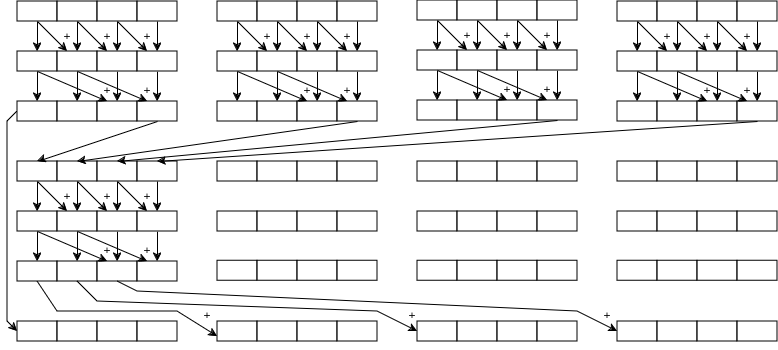
\includegraphics[width=0.8\textwidth]{img/warp-level-scan.png}
  \caption{\footnotesize Illustration of a warp-level inclusive scan with warp-size 4 and 16 threads}
  \label{fig:warpscan}
\end{figure}

To convert an inclusive to an exclusive scan, we shift the result to the right
by $1$ and insert the neutral element at the left-most position. Step 2.\ of
\textit{badd} use this warp-level exclusive scan with the operator $\otimes$ and
neutral element $\mathtt{e}$ defined in Equations (\ref{eq:otimesopt}),
(\ref{eq:otimesneopt}), and (\ref{eq:segscanop}).

What we have so far is enough to write \texttt{V1}, but \texttt{V2} and
\texttt{V3} requires some extra attention. We cannot directly use the warp-level
scan, because this works for one element per thread and we have $q$. Instead,
let us reuse the \textit{scan} $\shortrightarrow$ \textit{end-of-result}
$\shortrightarrow$ \textit{scan} $\shortrightarrow$ \textit{distribute} idea
from the warp-level scan algorithm on a register-level basis:

Let each thread compute the inclusive prefix sum of its $q$ elements
sequentially, and place only the last sum in shared memory. Then, run a
warp-level exclusive scan over the end-of-register-level sums in shared
memory. Lastly, each thread sequentially distribute the results of the
warp-level scan over the result of the register-level scan.

Using this idea, we are now able to write all three versions. For brevity, we
only show the main kernel body of \texttt{V3}, but both \texttt{V1} and
\texttt{V2} are principally implemented the same way. Listing \ref{addopcuda}
contains this kernel, where the input/output elements of each thread are read
coalesced beforehand and written coalesced afterwards to/from global memory.
\begin{lstlisting}[language=CPP,caption={\footnotesize
  CUDA \textit{badd} \texttt{V3} implementation body from file
  \texttt{ker-add.cu.h} (slightly edited), where registers \texttt{ass}, \texttt{bss}, and
  \texttt{rss} contains $q$ input/output digits, respectively, of type
  \texttt{uint\_t} with base class \texttt{Base}, segmented scan operator class
  \texttt{SegCarryProp} over carry type \texttt{carry\_t}, and shared memory
  buffer
  \texttt{shmem}.},label={addopcuda},firstnumber=212,gobble=4]
    const bool new_segm = threadIdx.x % (m/q) == 0;

    // 1. compute result, carry, register-level scan, and segment flags
    uint_t css[q];
    carry_t acc =
        new_segm ? SegCarryProp<Base>::setFlag(SegCarryProp<Base>::identity())
                 : SegCarryProp<Base>::identity();
    #pragma unroll
    for(int i=0; i<q; i++) {
        rss[i] = ass[i] + bss[i];
        css[i] = ((carry_t) (rss[i] < ass[i]))
                 | (((carry_t) (rss[i] == Base::HIGHEST)) << 1);
        acc = SegCarryProp<Base>::apply(acc, css[i]);
    }
    shmem[threadIdx.x] = acc;
    __syncthreads();

    // 2. propagate carries
    acc = scanExcBlock< SegCarryProp<Base> >(shmem, threadIdx.x);
    acc = new_segm ? SegCarryProp<Base>::identity() : acc;

    // 3. add carries to results
    #pragma unroll
    for(int i=0; i<q; i++) {
        rss[i] += (acc & 1);
        acc = SegCarryProp<Base>::apply(acc, css[i]);
    }
\end{lstlisting}

To reflect on the implementation; \cpp\ is verbose by design (as a C-like
language), and modelling the \textit{badd} algorithm requires care and
thought. Due to the nature of the CUDA extension, we furthermore have to reason
about the semantics in parallel, e.g.\ in the way we compute segment
beginnings. However, structuring the implementation around the high-level \cpp\
features of classes and templates, not only makes it generic and readable, but
also extensible in terms of optimizations. Once the fundamental version is
designed with proper usage of \cpp\ constructs, the optimizations comes as
natural extensions, while still allowing fine-grained control over the important
aspects, such as memory usage.

\subsection{Futhark Implementation}
\label{subsec:addfut}

In this section, we introduce four versions of addition in Futhark. The first
version (\texttt{V0}) is the original version formulated by Olesen et
al. \cite{DPPproject}, included for completeness. The second version
(\texttt{V1}) is the straightforward \textit{badd} algorithm.

The third version (\texttt{V2}) introduces a fixed sequentialization factor of
4, which we found to be the optimal factor from experimenting with the CUDA
implementation (see section \ref{subsec:addcud}). In CUDA, it is arbitrary to
make this factor generic using \cpp\ templates and compiler directives, without
loss of performance. In Futhark however, while we have type parameters and loop
unroll attributes, we do not have the fine-grained control of \cpp\ that allows
us to e.g. decide when and how to store intermediate results in shared
memory. We found that parameterizing the sequentialization factor is
significantly slower than fixing it. In turn, integers with size $m>4096$ does
not fit in a CUDA block, and requires manually increasing the factor. Another
approach could be to write a parameterized version for integers with $m>4096$,
and search for tricks that optimizes the compilers generated output. For
simplicity, we fix the factor at 4.

The fourth version (\texttt{V3}) introduces a parameterized number of instances
per block (\textit{ipb}) and the segmented \textit{badd}. This factor is fine to
vary, since it is only used to determine boolean values of the segmented
semantics.

Version \texttt{V0} and \texttt{V1} are defined straightforward, and due to
Futharks high-level design based on parallelism, they look almost identical to
the pseudocode of Figure \ref{fig:addpar}. E.g.\ Listing \ref{futaddv1} contains
the implementation of \texttt{V1}:
\begin{lstlisting}[language=futhark,caption={\footnotesize Futhark \textit{badd} \texttt{V1} using base \texttt{ui} and carry type \texttt{ct} (from file \texttt{add.fut} slightly edited).},label={futaddv1}]
def carryProp (c1: ct) (c2: ct) : ct =
  (c1 & c2 & 2) | (((c1 & (c2 >> 1)) | c2) & 1)

def carryPropE : ct = 2

def carryAug (r : ui) (a : ui) : ct =
  (boolToCt (r < a)) | ((boolToCt (r == HIGHEST)) << 1)

def baddV1 [m] (us: [m]ui) (vs: [m]ui) : [m]ui =
  -- 1. compute sums and carries
  let (ws, cs) = map2 (\ u v -> let w = u+v in (w, carryAug w u)) us vs
                 |> unzip
  -- 2. propagate carries
  let pcs = scanExc carryProp carryPropE cs
  -- 3. add carries to sums
  in map2 (\ w c -> w + fromCt (c & 1)) ws pcs
\end{lstlisting}

While versions \texttt{V0} and \texttt{V1} feeds into the strengths of Futhark
(simple abstract functions that run comparatively well), versions \texttt{V2} and
\texttt{V3} reveals the weaknesses. As mentioned, they include a fixed
sequentialization factor of 4, so we want to compute four sums for each
thread. It is therefore crucial that we pre-fetch the inputs to either shared or
register memory, greatly reducing the amount of reads from global memory (if
fetched coalesced). However, while easily done in our CUDA implementation, we
are at the mercy of the Futhark compiler to perform this optimization, and as of
writing this thesis, it does not.

Instead, we may exploit that the compiler stores intermediate arrays in shared
memory to e.g.\ read input $u$ into $w$ in a coalesced fashion. Normally, we
avoid such redundant computations because the compiler constructs and copies to
a new arrays when resolving array operations (, since data is immutable as per
usual for functional languages). However, the Futhark compiler use a memory
optimization strategy called array short-circuiting, where it performs a
short-circuit analysis that reveals whether it can skip constructing
intermediate arrays and execute the operation in-place instead
\cite{futhark/sc22mem}.

Thus, when we construct the read operation in a particular way, the compiler
will pre-allocate the inputs in shared memory when fused with the surrounding
functions, and in turn, generate the read operation with no-ops. We use the code
of Listing \ref{addfutcpy} below, which utilizes short-circuiting to read the
inputs into shared memory coalesced and with minimum overhead. I.e.\ the
\texttt{zip}s, \texttt{unzip}s and concatenations of the code becomes no-ops,
and \texttt{ush} and \texttt{vsh} is in-place read from \texttt{us} and
\texttt{vs} (occupying the same memory region).

\begin{lstlisting}[language=futhark,caption={\footnotesize Futhark code snippet reading
\texttt{us} and \texttt{vs} of size $\mathtt{ipb}\cdot \mathtt{m}$ from global to shared memory coalesced utilizing array short-circuiting (from file \texttt{add.fut} slightly
edited).},label={addfutcpy},gobble=2]
  let cp2sh (i : i32) = #[unsafe]
    let str = i32.i64 (ipb*m)
    in ((us[i], us[str + i], us[2*str + i], us[3*str + i])
       ,(vs[i], vs[str + i], vs[2*str + i], vs[3*str + i]))

  let (uss, vss) = (0..<ipb*m) |> map i32.i64 |> map cp2sh |> unzip
  let (u1s, u2s, u3s, u4s) = unzip4 uss
  let (v1s, v2s, v3s, v4s) = unzip4 vss
  let ush = u1s ++ u2s ++ u3s ++ u4s
  let vsh = v1s ++ v2s ++ v3s ++ v4s
\end{lstlisting}

The compiler attribute \texttt{\#[unsafe]} tells the compiler not to perform any
memory bound checks or optimizations. We generally add this attribute when a
sequentialization factor is involved, just to be certain that the compiler takes
our array indexing at face value.

Now, let us discuss the implementation of \texttt{V2} and \texttt{V3}. Their
type signature includes the shape parameters, enforcing the memory layout of the
inputs to be aligned:
\begin{lstlisting}[language=futhark,numbers=none,frame=,belowskip=-0.15 \baselineskip]
def baddV2 [m] (us: [4*m]ui) (vs: [4*m]ui) : [4*m]ui
def baddV3 [ipb][m] (us: [ipb*(4*m)]ui) (vs: [ipb*(4*m)]ui) : [ipb*(4*m)]ui
\end{lstlisting}
The functions are defined s.t.\ they first copy from global to shared memory (as
described above), and then run the function body (corresponding to the
\textit{badd} algorithm). For brevity, we focus on \texttt{V3} since they are
principally identical. The function body sequentializes the excess parallelism
using tuples of four elements as a manually unrolled loop. It exhibit the same
sequentialized register-level prefix sum approach as the CUDA \texttt{V3}
implementation of Listing \ref{addopcuda}. The function body is in Listing
\ref{futbaddv3} below.

\begin{lstlisting}[language=futhark,firstnumber=131,gobble=2,caption={\footnotesize Futhark \textit{badd} \texttt{V3} main function body using base \texttt{ui} and carry type \texttt{ct} from file \texttt{add.fut}.},label={futbaddv3}]
  let baddV3Run (us: []ui) (vs: []ui) : []ui = #[unsafe]
    -- 1. compute sums, carries, flags, and register-level prefix sum
    let (ws, cs, accs) = unzip3 <| imap (0..<ipb*m)
      (\ i -> let (u1, u2, u3, u4) = (us[i*4],us[i*4+1],us[i*4+2],us[i*4+3])
              let (v1, v2, v3, v4) = (vs[i*4],vs[i*4+1],vs[i*4+2],vs[i*4+3])
              let (w1, w2, w3, w4) = (u1 + v1, u2 + v2, u3 + v3, u4 + v4)
              let (c1, c2, c3, c4) = (carryAug w1 u1, carryAug w2 u2,
                                      carryAug w3 u3, carryAug w4 u4)
              let c1 = (boolToCt (i % m == 0)) << 2 | c1
              let acc = carryProp c1 <| carryProp c2 <| carryProp c3 c4
              in ((w1, w2, w3, w4), (c1, c2, c3, c4), acc))

    -- 2. propagate carries
    let pcs = scanExc carryPropSeg carryPropE accs

    -- 3. distribute carries over register-level prefix sum, and add to sum
    let (wi1s, wi2s, wi3s, wi4s) = unzip4 <| imap4 ws cs pcs (0..<ipb*m)
      (\ (w1, w2, w3, w4) (c1, c2, c3, _) acc1 i ->
         let acc1 = if i % m == 0 then carryPropE else acc1
         let acc2 = carryProp acc1 c1
         let acc3 = carryProp acc2 c2
         let acc4 = carryProp acc3 c3
         in ((w1 + fromCt (acc1 & 1), i*4),  (w2 + fromCt (acc2 & 1),i*4+1),
             (w3 + fromCt (acc3 & 1), i*4+2),(w4 + fromCt (acc4 & 1),i*4+3)))
    let (ws, inds) = unzip <| wi1s ++ wi2s ++ wi3s ++ wi4s
    in scatter (replicate (ipb*(4*m)) 0) inds ws
\end{lstlisting}

While \texttt{V2} and \texttt{V3} are still somewhat succinct, it is clear that
manipulating the compiler for certain optimizations introduces a lot more code
compared to the fundamentals of \texttt{V1}. This can especially become
cumbersome given the hand-written nature of the sequentialization factor. On the
other side, most of the Futhark code is still modelled closely to the algorithm,
and thus, making it easy to follow, reason about the semantics, and spot
potential errors.


\subsection{Subtraction}
\label{subsec:sub}

Subtraction is also a basic of arithmetic. Normally, we define subtracting by
adding the signed term. While we do not use signs in our underlying
representation, we can still define subtraction using the addition. In fact, it
is easy to see that the complement of each subroutine of the addition gives us
subtraction:

\begin{definition}[big integer subtraction]
  Subtraction of two big integers can be obtained from the generic algorithm of
  Figure \ref{fig:addpar}, where line 3 subtracts rather than adding the carry,
  and operators $\otimes$, $\mathtt{e}$, and $f$ remains the same as in
  \textit{badd}. The operator $\oplus$ then becomes:
\begin{align}
  \label{eq:oplussub}
  x \oplus y &\coloneq (x - y > x)~|~((x - y = 0) \ll 1)
\end{align}
\end{definition}

This definition has the usual unsigned integer wrap-around semantics. If we are
interested in the difference, we can check which input is the largest (by a
\texttt{map}-\texttt{reduce} composition), and then subtract and return the sign
accordingly.

Since it is the same algorithm as addition, we will not benchmark or discuss it
further.

%%% Local Variables:
%%% mode: LaTeX
%%% TeX-master: "../main"
%%% End:
